\documentclass[12pt]{beamer}
\usepackage{bookmark}
\usepackage[slovene]{babel}
\usepackage[utf8]{inputenc}
\usepackage{lmodern}
\usepackage[T1]{fontenc}
\usepackage{amsfonts,marvosym, amsthm}
\usepackage{amssymb,amsmath}


\usetheme{Boadilla}
\usecolortheme{whale}
\usefonttheme{professionalfonts}
\usepackage{etoolbox}
\setbeamertemplate{theorems}[nonumber]
\AtBeginEnvironment{theorem}{%
    \setbeamercolor{block title}{fg=white,bg=orange}
    \setbeamercolor{block body}{fg=black,bg=yellow}
}
\AtBeginEnvironment{proof}{%
    \setbeamercolor{block title}{fg=green,bg=red}
    \setbeamercolor{block body}{fg=black,bg=purple}
}

\setbeamercolor{normal text}{fg=black} 
% \usetheme{Frankfurt}
\usecolortheme{whale}
\theoremstyle{definition} % tekst napisan pokoncno
\newtheorem{definicija}{Definicija}[section]
\newtheorem{primer}[definicija]{Primer}
\newtheorem{opomba}[definicija]{Opomba}
\renewcommand\endprimer{\hfill$\diamondsuit$}
\theoremstyle{plain} % tekst napisan posevno
\newtheorem{lema}[definicija]{Lema}
\newtheorem{izrek}[definicija]{Izrek}
\newtheorem{trditev}[definicija]{Trditev}
\newtheorem{posledica}[definicija]{Posledica}
% za stevilske mnozice uporabi naslednje simbole
\newcommand{\R}{\mathbb R}
\newcommand{\N}{\mathbb N}
\newcommand{\Z}{\mathbb Z}
\newcommand{\C}{\mathbb C}
\newcommand{\Q}{\mathbb Q}


\title{Ravninske krivulje s pitagorejskim hodogramom}
\author{Tit Arnšek, Damijan Randl}
\date{Januar 2023}
\institute[Inst.]{Univerza v Ljubljani, Fakulteta za matematiko in fiziko \\ Geometrijsko podprto računalniško oblikovanje}
\date{Januar 2023}

\begin{document}

\begin{frame}
    \titlepage
\end{frame}

\begin{frame}
\begin{enumerate}
\item Ravninske krivulje s pitagorejskim hodografom
\item B\'ezierjeve kontrolne točke krivulj s PH
\item Parametrična hitrost in dolžina loka
\item Odvod krivulje 
\item Racionalni odmiki krivulj s PH
\end{enumerate}
\end{frame}

\begin{frame}
\frametitle{Ravninske krivulje s pitagorejskim hodografom}
\begin{itemize}
    \item PH krivulje
    \item Rida T. Farouki in Vangelis Sakkalis, 1990
    \item Uporaba v računalniško podprtem oblikovanju, proizvodnji (CNC razrez), robotiki, načrtovanju poti, animacijah... 
    \item Enostaven in natančen izračun dolžine; paralelne krivulje imajo racionalno parametrizacijo.
\end{itemize}
\centering

\includegraphics[width=4cm]{slika_1.jpeg}
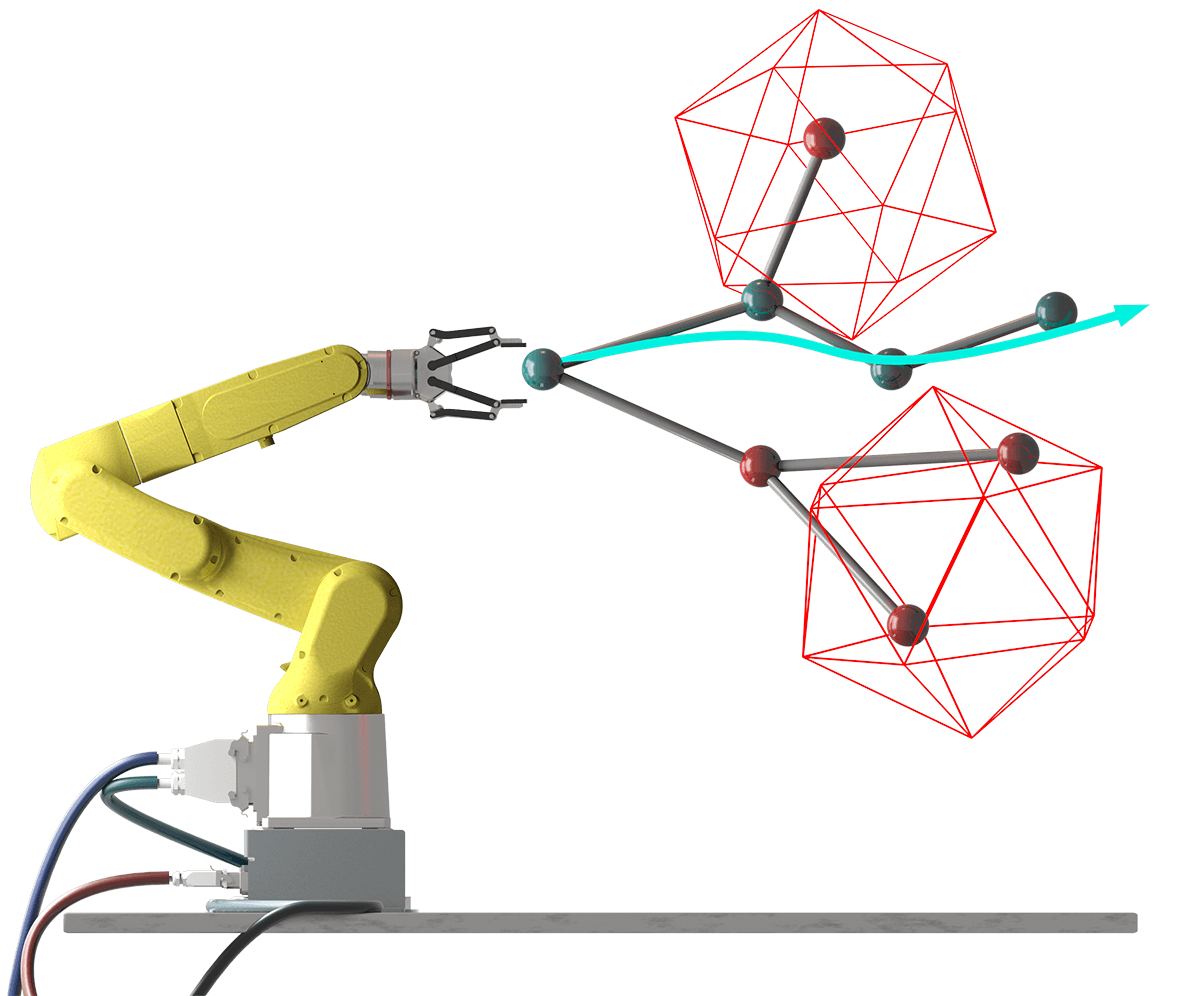
\includegraphics[width=4cm]{slika_2.png}
\end{frame}

\begin{frame}
    
    \begin{definicija}
        \begin{itemize}
            \item Hodograf odvedljive parametrične krivulje $r (t) = \begin{bmatrix} x(t) \\ y(t) \end{bmatrix} \in \mathbb{R}^2$ je definiran s predpisom $$r'(t) = \begin{bmatrix} x'(t) \\ y'(t) \end{bmatrix}.$$
            \item  Polinomska krivulja $r \in \mathbb{R}^2$ je krivulja s Pitagorejskim hodografom (PH), če velja naslednji pogoj:
            $$x'(t)^2 + y'(t)^2 = \sigma(t)^2 \text{ za nek polinom } \sigma.$$
        \end{itemize} 
    \end{definicija}
\end{frame}

\begin{frame}
    \begin{izrek}[Kubota]
        Polinomi $a$, $b$ in $c$ zadostijo pitagorejskemu pogoju
        $$a^2(t) + b^2(t) = c^2(t),$$
        natanko tedaj, ko jih lahko izrazimo s polinomi $u(t), v(t)$ in $w(t)$ v obliki
        $$a(t) = (u^2(t) - v^2(t))w(t),$$
        $$b(t) = 2u(t)v(t)w(t),$$
        $$c(t) = (u^2(t) + v^2(t))w(t),$$
        ter $u$ in $v$ nimata skupnih ničel.
        
    \end{izrek}

\end{frame}

\begin{frame}
    % \begin{itemize}
    %     \item $x'(t) = (u^2(t) - v^2(t))w(t),$
    %     \item $y'(t) = 2u(t)v(t)w(t),$
    %     \item $\sigma(t) = (u^2(t) + v^2(t))w(t),$
    % \end{itemize}
    \begin{opomba}
        \begin{itemize}
            \item  $w=0$ ali $u=v=0$, potem $r(t)$ predstavlja točko.
            \item $u$, $v$ in $w$ konstante in $w \neq 0$, vsaj eden od $u, v$ neničelna konstanta,
            potem $r(t)$ enakomerno parametrizirana daljica.
            \item $u$ in $v$ konstanti, $w$  ni konstanta, potem $r(t)$ neenakomerno parametrizirana daljica ali premica.
            \item $w = 0$ in $u = \pm v$ ali vsaj eden od $u, v$ ničelni polinom, 
            potem $r(t)$ neenakomerno parametrizirana daljica.
            \item $r(t)$ stopnje $n + 2m + 1$, kjer $n = deg(w)$ in $m = max(deg(u),deg(v))$
        \end{itemize} 
    \end{opomba}
      
\end{frame}

% \begin{frame}
% $ a^2 (t) + b^2 (t) = c^2 (t)$ natanko tedaj, ko obstajajo polinomi $u (t), v (t), w (t)$, tako da
% 		\begin{eqnarray} \label{eq:2}
% 		a (t) &=& \lbrack u^2(t)-v^2(t)\rbrack w(t),\nonumber\\
% 		b(t) &=& 2u(t)v(t)w(t),\\
% 		c(t) &=& \lbrack u^2(t)+v^2(t)\rbrack w(t),\nonumber
% 		\end{eqnarray}
% 		kjer imata $u(t)$ in $v(t)$ paroma različne ničle.
% \end{frame}

% \begin{frame}
% Ravninska krivulja s PH $r (t) = (x (t), y (t))$ definirana z zamenjavo treh polinomov $u (t), v (t), w (t)$ v izrazih
% 	\begin{eqnarray}\label{eq:3}
% 	x\prime(t) &=& \lbrack u^2(t)-v^2(t)\rbrack w(t)\\
% 	y\prime(t)&=&2u(t)v(t)w(t)\nonumber
% 	\end{eqnarray}
% 	in z integriranjem.
% \end{frame}

\begin{frame}
\frametitle{Kubične PH krivulje}
    \begin{itemize}
        \item Primitivni PH: $w=1$, $GCD(u, v) = konstanta$ % morda tudi max(deg(u), deg(v)) = 1
        \item Zapišimo $u$ in $v$ v Bernsteinovi bazi:
              $$ \textbf{u}(t) = u_0 B_0^1(t) + u_1 B_1^1(t) $$
              $$ \textbf{v}(t) = v_0 B_0^1(t) + v_1 B_1^1(t) $$
              Pri tem predpostavimo, da velja $u_0 : u_1 \neq v_0 : v_1$.
        \item Po zgornjem izreku tako dobimo hodograf
              $$\textbf{x}'(t) = (u_0^2 - v_0^2)B_0^2(t) + (u_0 u_1 - v_0 v_1) B_1^2(t) + (u_1^2 - v_1^2) B_2^2(t),$$
              $$\textbf{y}'(t) = 2 u_0 v_0 B_0^2(t) + (u_0 v_1 + u_1 v_0) B_1^2(t) + 2 u_1 v_1 B_2^2(t).$$
    \end{itemize}
\end{frame}
\begin{frame}
    \begin{itemize}
        \item Kubično PH krivljo tako zapišemo 
              $$ \textbf{r}(t) = (\textbf{x}(t), \textbf{y}(t))^T = \sum_{i=0}^{n}{\textbf{b}_k B_k^n(t)} $$
              kjer sta $x$ in $y$ izražena kot
              $$\textbf{x}(t) = \int_0^t (\textbf{u}^2(t) - \textbf{v}^2(t)) dt,$$
              $$\textbf{y}(t) = \int_0^t (2\textbf{u}(t)\textbf{v}(t))dt$$
        \item Pravilo za integriranje Bernstainovih baznih polinomov:
              $$\int B^n_i(t) dt = \frac{1}{n+1} \sum_{j=i+1}^{n+1} B^{n+1}_j(t)$$
    \end{itemize}
\end{frame}

\begin{frame}
    \begin{itemize}
        \item Integracija nam tako poda kontrolne točke kubične B\'ezierjeve krivulje
                \begin{eqnarray}
                    \textbf{b}_1 &=& \textbf{b}_0 + \frac{1}{3}(u_0^2 - v_0^2, 2 u_0 v_0)^T,\nonumber\\
                    \textbf{b}_2 &=& \textbf{b}_1 + \frac{1}{3}(u_0 u_1 - v_0 v_1, u_0 u_1 + v_0 v_1)^T,\nonumber\\
                    \textbf{b}_3 &=& \textbf{b}_2 + \frac{1}{3} (u_1^2 - v_1^2, 2 u_1 v_1)^T,\nonumber
                \end{eqnarray}
              Pri čemer je $\textbf{b}_0$ poljubna kontrolna točke, ki ustreza konstantam pri integraciji.
    \end{itemize}
\end{frame}

% \begin{frame}
% 	\begin{block}{}
% 		\begin{eqnarray}
% 			\textbf{p}_1 &=& \textbf{p}_0 + \frac{1}{5}(u_0^2-v_0^2,2u_0v_0),\nonumber\\
% 			\textbf{p}_2 &=& \textbf{p}_1 + \frac{1}{5}(u_0u_1-v_0v_1,u_0v_1+u_1v_0),\nonumber\\	
% 			\textbf{p}_3 &=& \textbf{p}_2 + \frac{2}{15}(u_1^2-v_1^2,2u_1v_1)+\nonumber\\
% 			& & \frac{1}{15}(u_0u_2-v_0v_2,u_0v_2+u_2v_0),\nonumber\\
% 			\textbf{p}_4 &=& \textbf{p}_3 + \frac{1}{5}(u_1u_2-v_1v_2,u_1v_2+u_2v_1),\nonumber\\
% 			\textbf{p}_5 &=& \textbf{p}_4 + \frac{1}{5}(u_2^2-v_2^2,2u_2v_2),\nonumber
% 		\end{eqnarray}
% 	\end{block}	
% \end{frame}

\begin{frame}
\frametitle{Parametrična hitrost in dolžina loka}
Parametrična hitrost:
$$ | r\prime (t) | =\sqrt{x\prime^2(t)+y\prime^2(t)}= u^2 (t) + v^2 (t) = \sigma (t)$$
$$\sigma (t) =\sum_{k=0}^{n-1} \sigma_kB_k^{n-1}(t),$$
	kjer  
$$\sigma_k =\sum_{j=max(0,k-m)}^{min(m,k)}\frac{\binom{m}{j}\binom{m}{k-j}}{\binom{n-1}{k}}(u_ju_{k-j}+v_jv_{k-j}),$$ $$k = 0,\ldots , n - 1.$$
\end{frame}
\begin{frame}
    Dolžina loka:
    $$s (t) =\int^t_0\sigma(\tau) d\tau,$$
    $$s (t) =\sum^n_{k=0}s_k\binom{n}{k}(1-t)^{n-k}t^k=\sum_{k=0}^n s_kB^n_k(t),$$
	kjer  $$s_0=0 \quad \text{in} \quad s_k=\frac{1}{n}\sum^{k-1}_{j=0}\sigma_j \quad k=1,\ldots,n.$$

    Skupna dolžina loka je $S(1)$. 
    \newline
    
    Enotska tangenta in normala:
    $$\textbf{t} =\frac{(u^2 - v^2, 2uv)}{\sigma} \quad \quad
     \textbf{n} =\frac{(2uv, v^2 - u^2)}{\sigma}$$
\end{frame}
% \begin{frame}
% \begin{block}{}
% 	\begin{eqnarray}
% \sigma_0 &=& u^2_0+ v^2_0, \nonumber\\
% 	\sigma_1 &=& u_0u_1 + v_0v_1, \nonumber\\
% 	\sigma_2 &=& u^2_1+ v^2_1.\nonumber
% 	\end{eqnarray}
% \end{block}
% \begin{block}{}
% 	\begin{eqnarray}
% 	\sigma_0&=&u_0^2+v_0^2,\nonumber\\
% 	\sigma_1&=&u_0u_1+v_0v_1,\nonumber\\
% 	\sigma_2&=&\frac{2}{3}(u_1^2+v_1^2)+\frac{1}{3}(u_0u_2+v_0v_2),\nonumber\\
% 	\sigma_3&=&u_1u_2+v_1v_2,\nonumber\\
% 	\sigma_4&=&u_2^2+v_2^2.\nonumber
% 	\end{eqnarray}
% \end{block}
% \end{frame}
	
% \begin{frame}
% $$s (t) =\sum_{k=0}^n s_kB^n_k(t),$$
% 	kjer je $s_0=0$ in $s_k=\frac{1}{n}\sum^{k-1}_{j=0}\sigma_j, k=1,\ldots,n.$
% \begin{block}{}
% $S = s (1) = \frac{\sigma_0+\sigma_1+\ldots+\sigma_{n-1}}{n}.$
% \end{block}
% \end{frame}

% \begin{frame}
% $\Delta s = S / N$

% Začetni približek: $$t^{(0)}_k = t_{k-1}+\frac{\Delta s}{\sigma(t_{k-1})}$$
% Newton-Raphson:
% $$t^{(r)}_k = t^{(r-1)}_k-\frac{s(t^{(r-1)}_k)-k\Delta s}{\sigma(t^{(r-1)}_k)}, r = 1, 2,\ldots.$$
% \end{frame}
	
	
% 	\begin{frame}
% 	\frametitle{Lastnosti odvoda krivulje}
% 	$$\textbf{t} =\frac{(u^2 - v^2, 2uv)}{\sigma}$$ $$\textbf{n} =\frac{(2uv, v^2 - u^2)}{\sigma}$$ $$\kappa = 2 \frac{uv\prime - u\prime v}{\sigma^2}.$$
% \end{frame}
	

% \begin{frame}
% 	\frametitle{Racionalni odmiki krivulj s PH}
% \only<1>{$$r_d (t) = r (t) + d \textbf{n} (t),$$ kjer je $\textbf{n} (t)$ enotska normala .}
% \pause
% $$\textbf{P}_k = (W_k, X_k, Y_k) = (1, x_k, y_k),\hspace{20pt} k = 0,\ldots , n.$$
% $$\Delta\textbf{P}_k = \textbf{P}_{k + 1} - \textbf{P}_k = (0, \Delta x_k, \Delta y_k),\hspace{20pt} k = 0,\ldots, n - 1$$
% $$\Delta\textbf{P}_k^\perp = (0, \Delta y_k, -\Delta x_k).$$
% \pause
% \begin{block}{Racionalni odmik}
% $$r_d (t) = \left(\frac{X (t)}{W(t)},\frac{Y(t)}{W(t)}\right),$$
% kjer je $\textbf{O}_k = (W_k, X_k, Y_k), \hspace{10px} k = 0,\ldots , 2n - 1,$ določeno z
% $$\textbf{O}_k =\sum^{min (n - 1, k)}_{j = max (0, k - n)}\frac{\binom{n-1}{j}\binom{n}{k-j}}{\binom{2n-1}{k}}(\sigma_j\textbf{P}_{k-j}+dn\Delta\textbf{P}_j^\perp).$$
% \end{block}
% \end{frame}

\begin{frame}
    \frametitle{Racionalni odmik PH krivulje}
        \begin{itemize}
            \item Odmik krivulje $\textbf{r}(t)$ na razdalji $d$ je definiran kot 
                  $$\textbf{r}_d(t) = \textbf{r}(t) + d \textbf{n}(t)$$
            \item Racionalni odmik PH krivulje lahko predstavimo kot:
                  $$ \textbf{r}_d(t) = \left(\frac{X(t)}{W(t)}, \frac{Y(t)}{W(t)}\right)$$ 
            \item Kontrolne točke paralelne racionalne PH krivulje:
                  $$\textbf{O}_k = \sum_{j=\max(0, k-n)}^{\min(n-1, k)} \frac{\binom{n-1}{j} \binom{n}{k-j}}{\binom{2n-1}{k}}(\sigma_j \textbf{P}_{k-j}+ d n \Delta\textbf{P}^\perp_j),$$ 
                  $$k=0, ..., 2n-1$$
        \end{itemize}

    \end{frame}
    \begin{frame}
        \begin{itemize}
            \item Racionalni odmik kubične PH krivulje je 5. stopnje
            \item Homogeni zapis koordinat kontrolnih točk PH krivulje \textbf{r}(t):
                  $$ \textbf{P}_k = (W_k, X_k, Y_k) = (1, x_k, y_k), \quad k = 0, ..., n$$
            \item Pri tem so
                  $$\textbf{O}_k = (W_k, X_k, Y_k), k = 0, ..., 2n-1$$
                  kontrolne točke racionalnega odmika.
            
        \end{itemize}
    \end{frame}
    
    \begin{frame}
        \begin{itemize}
            \item Tako dobimo kontrolne točke racionalnega odmika kubične PH krivulje:
                \begin{eqnarray}
                    \textbf{O}_0 &=& \sigma_0 \textbf{P}_0 + 3 d \Delta \textbf{P}_0^{\perp},\nonumber \\
                    \textbf{O}_1 &=& \frac{1}{5} [2 \sigma_1 \textbf{P}_0 + 3\sigma_0 \textbf{P}_1 + 3 d (3 \Delta \textbf{P}_0^{\perp} + 2 \Delta \textbf{P}_1^{\perp})],\nonumber \\
                    \textbf{O}_2 &=& \frac{1}{10} [\sigma_2 \textbf{P}_0 + 6\sigma_1 \textbf{P}_1 + 3\sigma_0 \textbf{P}_2 + \nonumber \\
                        & & 3 d (3 \Delta \textbf{P}_0^{\perp} + 6 \Delta \textbf{P}_1^{\perp} + \Delta \textbf{P}_2^{\perp})],\nonumber \\
                    \textbf{O}_3 &=& \frac{1}{10} [3\sigma_2 \textbf{P}_1 + 6\sigma_1 \textbf{P}_2 + \sigma_0 \textbf{P}_3 + \nonumber \\
                        & & 3 d (\Delta \textbf{P}_0^{\perp} + 6 \Delta \textbf{P}_1^{\perp} + 3 \Delta \textbf{P}_2^{\perp})],\nonumber \\
                    \textbf{O}_4 &=& \frac{1}{5} [3\sigma_2 \textbf{P}_2 + 2\sigma_1 \textbf{P}_3 + 3 d (2\Delta \textbf{P}_1^{\perp} + 3 \Delta \textbf{P}_2^{\perp})],\nonumber \\
                    \textbf{O}_5 &=& \sigma_2 \textbf{P}_3 + 3 d \Delta \textbf{P}_2^{\perp}\nonumber
                \end{eqnarray}
                
        \end{itemize}
    \end{frame}

\end{document}